\documentclass{article}

\setlength{\headsep}{0.75 in}
\setlength{\parindent}{0 in}
\setlength{\parskip}{0.1 in}

\usepackage{xcolor}
\usepackage[margin=1in]{geometry} % Used for page margins, often replaces fullpage
\usepackage{amsmath,amsthm,amssymb} % amssymb added for common math symbols

\usepackage{enumitem}
\usepackage{tikz}

\usepackage{algorithm}
\usepackage{algpseudocode}
\usepackage{enumitem}

\title{Assignment 2: Search Problems in AI}
\author{Joaquin Pollard, Ammar Ghauri}
\date{\today}

\begin{document}

\maketitle

\section*{Problem 1}
Trace the operation of $A^*$ search (use the tree version, i.e. without using a closed list) applied to
the problem of getting to Bucharest from Lugoj using the straight-line distance heuristic. That is, show the sequence of
nodes that the algorithm will consider and the $f$ , $g$, and $h$ score for each node. You don’t need to draw the graph, just right
down a sequence of $(city, f (city), g(city), h(city))$ in the order in which the nodes are expanded.

\begin{center}
   \textbf{find the sequence of cities expanded (Lugoj $\rightarrow$  Bucharest)}\\
   $f(n) = g(n) + h(n)$
\end{center}
With $g(n)$ distance from Lugoj and $h(n)$ straight-line distance to Bucharest

\textbf{ANSWER:}

\begin{enumerate}
   \item $(city, f(city), g(city), h(city))$
   \item (Lugoj, 244, 0, 244)
   \begin{itemize}
      \item (Timisoara, 111, 329, 440)
      \item \textbf{(Mehadia, 311, 70, 241) $\rightarrow$ expand this due to lower $f$ value}
   \end{itemize}
   \item (Mehadia, 311, 70, 241)
   \begin{itemize}
      \item \textbf{(Lugoj, 384, 140, 244) $\rightarrow$ expand this again since it has lower $f$ value}
      \item (Drobeta, 387, 145, 242)
   \end{itemize}
   \item (Lugoj, 384, 140, 244)
   \begin{itemize}
      \item (Timisoara, 580, 251, 329) 
      \item (Mehadia, 451, 210, 241) 
      \item So we expand the next closest which is \textbf{Drobeta}.
   \end{itemize}
   \item (Drobeta, 387, 145, 242)
   \begin{itemize}
      \item (Mehadia, 461, 220, 241)
      \item \textbf{(Craiova, 425, 265, 160) $\rightarrow$ expand this one}
   \end{itemize}
   \item (Craiova, 425, 265, 160)
   \begin{itemize}
      \item (Drobeta, 625, 385, 242)
      \item (Rimnicu Vilcea, 604, 411, 193)
      \item \textbf{(Pitesti, 503, 403, 100) $\rightarrow$ expand this next}
      \item We just expand the previously visited cities to traverse any other possible routes
   \end{itemize}
   \item (Timisoara, 440, 111, 329)
   \begin{itemize}
      \item (Arad, 595, 229, 366)
      \item (Lugoj, 466, 222, 244)
   \end{itemize}
   \item (Mehadia, 451, 210, 241)
   \begin{itemize}
      \item (Lugoj, 524, 280, 244)
      \item (Drobeta, 527, 285, 242)
   \end{itemize}
   \item (Mehadia, 461, 220, 241)
   \begin{itemize}
      \item (Lugoj, 534, 290, 244)
      \item (Drobeta, 537, 295, 242)
   \end{itemize}
   \item (Lugoj, 466, 222, 244)
   \begin{itemize}
      \item (Timisoara, 662, 333, 329)
      \item (Mehadia, 533, 292, 241)
   \end{itemize}
   \item (Pitesti, 503, 403, 100) 
   \begin{itemize}
      \item (Rimnicu Vilcea, 693, 500, 193)
      \item (Craiova, 701, 541, 160)
      \item \textbf{(Bucharest, 504, 0, 504) $\rightarrow$ goal city is reached!}
   \end{itemize}
   \item (Bucharest, 504, 504, 0)
\end{enumerate}




\section*{Problem 2}
Consider a state space where the start state is number 1 and each state $k$ has two successors:
numbers $2k$ and $2k + 1$
\begin{itemize}
   \item Suppose the goal state is 11. List the order in which states will be visited for breadthfirst search, depth-limited search with limit 3, and iterative deepening search.
\end{itemize}

\begin{tikzpicture}[
    every node/.style={circle, draw, minimum size=1em},
    level 1/.style={sibling distance=4cm, level distance=1.5cm},
    level 2/.style={sibling distance=2cm, level distance=1.5cm},
    level 3/.style={sibling distance=1cm, level distance=1.5cm}
]

\node{1}
    child {node{2}
        child {node{4}
            child {node{8}}
            child {node{9}}
        }
        child {node{5}
            child {node{10}}
            child {node{11}}
        }
    }
    child {node{3}
        child {node{6}}
        child {node{7}}
    };

\end{tikzpicture}
\begin{center}
   \textbf{So it goes through each number until goal state (11) is reached}
\end{center}
\begin{center}
   Visited: 1$\rightarrow$2$\rightarrow$3$\rightarrow$4$\rightarrow$5$\rightarrow$6$\rightarrow$7$\rightarrow$8$\rightarrow$9$\rightarrow$10$\rightarrow$11
\end{center}

depth 0: 1\\
depth 1: 2$\rightarrow$3\\
depth 2: 4$\rightarrow$5$\rightarrow$6$\rightarrow$7\\
depth 3: 8$\rightarrow$9$\rightarrow$10$\rightarrow$11

\begin{itemize}
   \item How well would bidirectional search work on this problem? List the order in which states will be visited. What is the branching factor in each direction of the bidirectional search?
\end{itemize}

\begin{center}
   * With binary search, we start from initial state and also from the goal state then stop when both searches at the same node *
\end{center}

\textbf{Forward Search} $\rightarrow$ from initial state\\
- branching factor: 2k, 2k + 1 (Since each node produces two "children")
node 1: 2,3\\
node 2: 4,5\\
node 3: 6,7\\
node 4: 8,9\\
node 5: 10,11\\
\begin{center}
   Forward expansion: 1$\rightarrow$2$\rightarrow$3$\rightarrow$4$\rightarrow$5
\end{center}

\medskip

\textbf{Backward Search} $\rightarrow$ from goal state\\
- branching factor: ($\frac{k}{2}$) since each child node only has one parent node \\ 
node 11: 5\\
node 5: 2\\
node 2: 1 \\

\begin{center}
   Backward expansion: 11$\rightarrow$5
\end{center}

\textbf{Conclusion:} bidirectional search is much better since it can simply traverse through the tree since the 
Backward search has a branching factor of 1 that can simply go from 11$\rightarrow$5$\rightarrow$2$\rightarrow$1. 



\section*{Problem 3}
Which of the following statements are correct and which ones are wrong? 
\begin{enumerate}
   \item[(a)] This is correct since Uniform-cost search expands the node with the lowest path cost. If all steps costs are similar, then the smallest $g(n)$ reflects to the shallowest node.
   \item[(b)] This is false since DFS uses a stack that expands the deepest node, not the one with smallest $f$ which what best-fit search does.
   \item[(c)] This is correct since A* uses $f(n) = g(n) + h(n)$ and if $h(n)$ = 0, then $f(g) = g(n)$. This is exactly uniform-cost search.
   \item[(d)] This is not true since is goes long way path first. 
   \item[(e)] This is only true if all edges cost the same, if not, then it's false. 
   \item[(f)] This is true since uniform-cost search always expands the lowest path cost
   \item[(g)] This is true when there's consiste heuristic since it guarantees $h(n) \leq c(n, n') + h(n')$
   \item[(h)] This is false because there's no guarantee A* expands fewer nodes than DFS
   \item[(i)] If heuristic is consistent, then A* will either expand fewer or the same as uniform-cost search, so this is true. 
\end{enumerate}

\section*{Problem 4} Iterative deepening is sometimes used as an alternative to breadth first search. Give one advantage
of iterative deepening over BFS, and give one disadvantage of iterative deepening as compared with BFS. Be concise and
specific.
\medskip

\textbf{ADVANTAGE} 
\newline
- Iterative deepening traverses a tree by examining the depth levels rather than iterating the whole nodes when searching for a goal state.\\
- With doing so, this reduces the amount of space it takes up compared to BFS which has to go through a whole path of nodes from initial to goal state.\\
- Therefore, iterative deepening only stores the current DFS path ($O(bd)$) rather than storing all nodes which can take $O(b^d)$ space.\\
\begin{center}
   \textbf{Since $O(bd) < O(b^d)$, Iterative deepening takes less space than BFS.}
\end{center}

\textbf{DISADVANTAGE}\\
- However, if the goal state is large, the depth searched also increases.\\
- BFS only expands each node ones no matter how large the nodes are.\\
- This makes iterative deepening to re-expand nodes multiple times more than BFS.\\
- This causes iterative deepening to have extra computational time compared to BFS.\\
- For example, from problem 2's tree with an initial state of 1 and goal state of 11:
\begin{itemize}
   \item \textbf{BFS} traverses the node 
   \begin{itemize}
      \item 1
      \item 2,3
      \item 4,5,6,7
      \item 8,9,10,11
   \end{itemize}
   \item Each node is only expanded \textbf{ONCE}
   \item On the other hand, Iterative deepening expands: 
   \begin{itemize}
      \item 1
      \item 1,2,3
      \item 1,2,4,5,3,6,7
      \item 1,2,4,8,9,5,10,11
   \end{itemize}
   \item In this case, (1,2,4, and 5) were expanded \textbf{TWICE}
   \item This shows that iterative deepening waste time for re-expanding previously expanded nodes.
\end{itemize}


\section*{Problem 5}
Prove that if a heuristic is consistent, it must be admissible. Construct an example of an admissable heuristic that is not consistent.
(Hint: you can draw a small graph of 3 nodes and write an arbitrary cost and heuristic values so that that the heuristic is admissable but not consistent).
\medskip
\textbf{ANSWER}\\

\begin{center}
   a heuristic $h(n)$ is consistent for every edge n $\rightarrow$ n'\\
   $h(n) \le c(n,n') + h(n')$ with $h(goal state) = 0$
\end{center}

- Assume the most optimal path from node n to goal is $n_1 \rightarrow n_2 \rightarrow n_3 \rightarrow \cdot\cdot\cdot \rightarrow goal$\\
- and each cost $c(n, n_1), c(n, n_2), \cdot\cdot\cdot c(n, n_n)$\\
- We can apply the consistency repeatedly 
\begin{enumerate}
   \item $h(n) \le c(n,n_1) + h(n_1)$
   \item $h(n_1) \le c(n_1,n_2) + h(n_2)$
   \item until $h(n) \le c(n,n_1) + c(n, n_2) + \cdot\cdot\cdot + c(n_k, goal state) + h(goal state)$
\end{enumerate}
* Since h(goal) = 0, we aim to obtain h(n) $\le$ true cost to the goal. This causes the heuristic to never overestimate and is admissible.

\textbf{For Example:}

\begin{center}

\begin{tikzpicture}[node distance=2.5cm, every node/.style={circle, draw}]
\node (A) {A};
\node (B) [right of=A] {B};
\node (C) [right of=B] {C};

\draw[->] (A) -- node[above]{1} (B);
\draw[->] (B) -- node[above]{1} (C);
\end{tikzpicture}
\end{center}

True shortest costs to the goal:

$h^*(A) = 2, \quad h^*(B) = 1, \quad h^*(G) = 0$


Define the heuristic:

$h(A)=2, \quad h(B)=0, \quad h(G)=0$


This heuristic is \textbf{admissible} since

$h(A) \le 2, \quad h(B) \le 1, \quad h(G) \le 0$

However, it is \textbf{not consistent} because

$h(A) > c(A,B) + h(B)$

2 $>$ 1 + 0 \\

\begin{center}
   The heuristic is admissible but not consistent since it goes against the consistency condition.
\end{center}







\section*{Problem 6}
In a CSP search problem, it is better to choose the variable that is most constrained and the value that is least constraining because it reduces the search space and increases the likelihood of finding a valid assignment quickly. If one selects the most constrained variable(Minimum Remaining Values heuristic), that means he will choose the variable with the fewest legal values remaining(detecting failure early). In the case a variable does not have any valid assignments left, the algorithm can backtrack instead of exploring deeper into an invalid branch. Upon selecting the variable, choosing the least constraining value means one selects the value that eliminates the least amount of options for the remaining unassigned variables. This will come in use for future assignments as it preserves and reduces the probability of conflicts later on in the search.

\section*{Problem 7}
\textbf{(a) Best move using minimax}

First move made by MAX at node $A$, and the next level corresponds to MIN nodes.

Left subtree:

\[
D = 3, \quad E = 5
\]

Since $B$ is a MIN node:

\[
B = \min(3,5) = 3
\]

Right subtree:

Node $F$ is a MIN node with children $I$ and $J$.

\[
I = \max(0,7) = 7
\]

\[
F = \min(7,5) = 5
\]

Node $G$ is a MIN node:

\[
G = \min(7,8) = 7
\]

Node $H = 4$

Node $C$ is a MIN node:

\[
C = \min(5,7,4) = 4
\]

Finally, MAX selects:

\[
A = \max(3,4) = 4
\]

Therefore, the best move for MAX is to choose node $C$.

\bigskip

\textbf{(b) Alpha-Beta Pruning (Left-to-Right)}

\begin{tikzpicture}[
    every node/.style={circle, draw, minimum size=1em},
    level 1/.style={sibling distance=4cm, level distance=1.5cm},
    level 2/.style={sibling distance=2cm, level distance=1.5cm},
    level 3/.style={sibling distance=1.5cm, level distance=1.5cm},
    level 4/.style={sibling distance=1cm, level distance=1.5cm}
]

\node{A}
    child {node{B}
        child {node{D}}
        child {node{E}}
    }
    child {node{C}
        child {node{F}
            child {node{I}
                child {node{M}}
            }
            child {node{J}}
        }
        child {node{G}
            child {node{K}}
        }
        child {node{H}}
    };

\end{tikzpicture}

\textbf{(c) Alpha-Beta Pruning (Right-to-Left)}

\begin{tikzpicture}[
    every node/.style={circle, draw, minimum size=1em},
    level 1/.style={sibling distance=4cm, level distance=1.5cm},
    level 2/.style={sibling distance=2cm, level distance=1.5cm},
    level 3/.style={sibling distance=1.5cm, level distance=1.5cm}
]

\node{A}
    child {node{B}
        child {node{D}}
        child {node{E}}
    }
    child {node{C}
        child {node{F}
            child {node{J}}
        }
        child {node{G}
            child {node{L}}
        }
        child {node{H}}
    };

\end{tikzpicture}






Because alpha-beta pruning is highly dependent on the order in which nodes are explored, different pruning occures. When good moves are evaluated earlier, tighter bounds will be established sooner, allowing for more branches to be pruned.
\section*{Problem 8}
Which of the following are consistent?

We know a heuristic is consistent if

h(n) \le c(n,n') + h(n')

for every edge. Given that h_1 and h_2 are consistent:

a) h(n) = \min\{h_1(n), h_2(n)\}

Because

h_1(n) \le c(n,n') + h_1(n')  
h_2(n) \le c(n,n') + h_2(n')

the minimum of the two also satisfies the inequality. So

\min\{h_1(n), h_2(n)\} \le c(n,n') + \min\{h_1(n'), h_2(n')\}

Therefore, a is consistent.

b) h(n) = w h_1(n) + (1 - w) h_2(n)

Using consistency of h_1 and h_2:

h_1(n) \le c(n,n') + h_1(n')  
h_2(n) \le c(n,n') + h_2(n')

Multiply by the weights and add:

w h_1(n) + (1 - w) h_2(n)
\le w(c(n,n') + h_1(n')) + (1 - w)(c(n,n') + h_2(n'))

= c(n,n') + w h_1(n') + (1 - w) h_2(n')

= c(n,n') + h(n')

Therefore, b is also consistent.

c) h(n) = \max\{h_1(n), h_2(n)\}

Since

h_1(n) \le c(n,n') + h_1(n')  
h_2(n) \le c(n,n') + h_2(n')

taking the maximum preserves the inequality:

\max\{h_1(n), h_2(n)\} \le c(n,n') + \max\{h_1(n'), h_2(n')\}

Therefore, c is also consistent.

a consistent  
b consistent  
c consistent


Which of the following are admissible?

We know a heuristic is admissible if

h(n) \le h^*(n)

for every node, where h^*(n) is the true optimal cost from n to the goal. Given that h_1 and h_2 are admissible:

a) h(n) = \min\{h_1(n), h_2(n)\}

Because

h_1(n) \le h^*(n)  
h_2(n) \le h^*(n)

the minimum of the two is also less than or equal to h^*(n). So

\min\{h_1(n), h_2(n)\} \le h^*(n)

Therefore, a is admissible.

b) h(n) = w h_1(n) + (1 - w) h_2(n), where 0 \le w \le 1

Using admissibility of h_1 and h_2:

h_1(n) \le h^*(n)  
h_2(n) \le h^*(n)

Multiply by the weights and add:

w h_1(n) + (1 - w) h_2(n)
\le w h^*(n) + (1 - w) h^*(n)

= h^*(n)

Therefore,

h(n) \le h^*(n)

So b is admissible.

c) h(n) = \max\{h_1(n), h_2(n)\}

Since

h_1(n) \le h^*(n)  
h_2(n) \le h^*(n)

the maximum of the two is still less than or equal to h^*(n). So

\max\{h_1(n), h_2(n)\} \le h^*(n)

Therefore, c is admissible.

a admissible  
b admissible  
c admissible

\section*{Problem 9}
a. Hill climbing is better than simulated annealing when every uphill path naturally leads to the global maximum, or at least when local search traps are rare. In that type of problem, always moving uphill is considered enough. Therefore random “bad-move” made by simulated annealing is unnecessary overhead.

b. The hill climbing part of simulated annealing is not necessary when the objective landscape is so noisy/uninformative that local moves do not give you reliable signs of improvement. Being near good states does not necesitate that you are likely to find an even better one near it.

c. Simulated annealing is useful in problems where the landscape has useful/insignful local structure. It doesnt necesitate that the value function is perfectly smooth or completely random, but that there is enough structure for local improvement to matter and enough local traps that some randomness is needed to escape them.

d. Instead of just returning the final state something we could adjust would be to keep track of and return the best encountered state during the search as simulated annealing may move on away from them (the good states) as it explores.

e. If we had the capacity to store two million states, we could potentially maintain very good candidate states and explore multiple regions of the search space in parallel. We could then share information about good states instead of running independent simulated annealing runs.

f. Gradient ascent always moves in the directions of the steepest increase making it prone to getting stuck in local maxima. We could potentially introduce a temperature controlled probability of taking downhill steps so the algorithm can escape local maxima early in the search. This will help it to gradually behave like standard gradient ascent as temperature decreases.


\end{document}
